\chapter{Temperature fitting}
The results of the EPOCH simulations provide weighted momenta of electrons $\bm{p}_\mathrm{e}$, where the weight represents the number of electrons with that momentum. They are not histograms yet, because more than one macro-particle can be assigned with the same value of $\bm{p}_\mathrm{e}$. The energies of electrons can then be calculated from $\bm{p}$ using the relativistic formula:
\begin{equation}
	\label{eq:rel-energy}
	E_\mathrm{e} = m_0\cdot c^2\left(\sqrt{1+\left(\frac{p}{m_0\cdot c}\right)^2} -1\right)\mathrm{,}
\end{equation}
where $p=\sqrt{\bm{p}\cdot\bm{p}}$, $m_0 =  9.109 \cdot 10^{-31} \, \mathrm{kg}$ is the electron rest-mass and $c=3\cdot 10^{8} \, \mathrm{m . s}^{-1}$ is the speed of light \cite{constants}.


\begin{figure}[h]
	\centering
	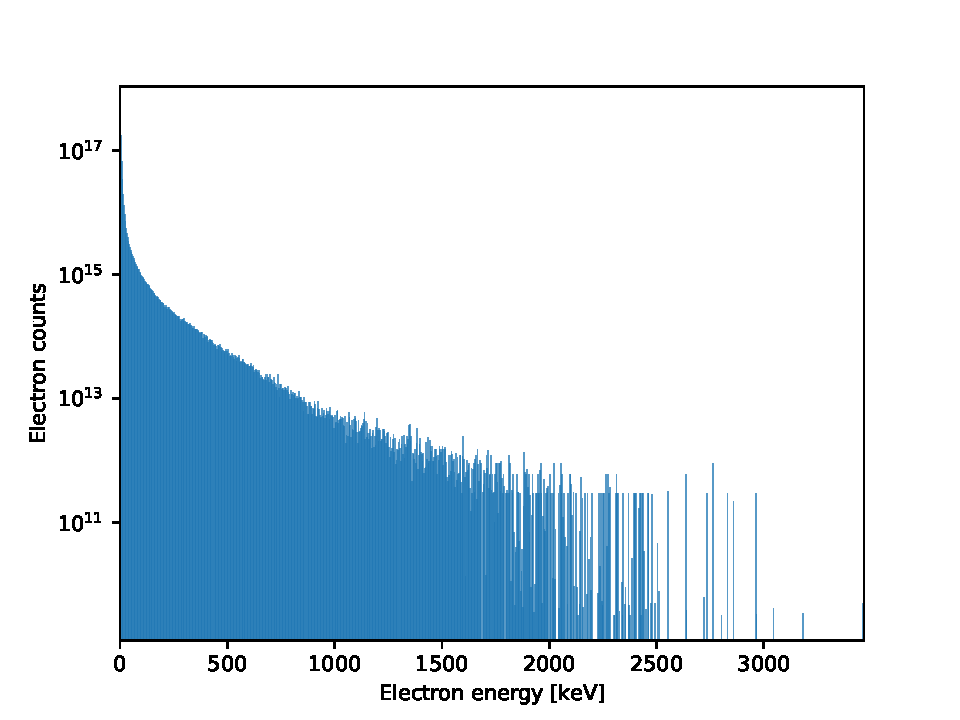
\includegraphics[width=0.7\textwidth]{figures/example-histogram}
	\caption{An example of electron energy distribution of 2D EPOCH simulation with intensity of laser $I=10^{19}\,\mathrm{W.cm}^{-2}$, characteristic scale of the exponential preplasma profile $L=0.1\,\mathrm{\mu m}$ and angle of incidence with respect to target normal direction $\alpha = 10$°.}
	\label{fig:example-histogram}
\end{figure}
After using equation \ref{eq:rel-energy} to calculate energy, it is multiplied by the weight. One can easily create the histogram from electron energies and their counts. An example of such histogram can be seen in the figure \ref{fig:example-histogram}. There are several things that need to be discussed.

It is important to note that the $y$-axis is presented on a logarithmic scale to enhance readability. The extensive range of electron energies necessitates the use of relativistic formula. However, around the energies $E_k \approx 1900 \, \mathrm{keV}$ and more, the histogram exhibits irregularities - specifically, there are empty bins and several bins contain identical electron counts. These anomalies are attributed to the EPOCH weighting process. Consequently, this portion of the spectrum is rendered questionable. This issue will be further addressed in the section dedicated to temperature fitting.

Last but not least, note the apparent exponential relationship between $N_i$ and $E_k$ in the energy spectrum between $E_k \approx 500 \, \mathrm{keV}$ and $E_k \approx 1500 \, \mathrm{keV}$:
\begin{equation}
	\label{eq:exp-distr}
	N_i = N_0 \cdot \mathrm{exp}\left( -\frac{E_i}{T}\right)\mathrm{,}
\end{equation}
where $N_i$ is count in $i$-th bin and $E_i$ is the corresponding energy and $T$ is temperature in units discussed in section \ref{sec:temperature-intro}. The relationship, of course, linear in logarithmic scale. The equation of \ref{eq:exp-distr} resembles exponential distribution with $1/T$ missing on the right-hand side. It is also not normalized, because it represents counts that have to add up to total number of electrons with that temperature. For the purpose of this thesis, we will call it the \textit{Boltzmann distribution}, even though it is not completely accurate.

Fitting the correct part of the histogram using equation \ref{eq:exp-distr} and estimating $T$ and $N_0$ is the first bigger part of this thesis. There are several obstacles, all of which are discussed in following sections.

\section{Boltzmann vs. Maxwellian distribution}
First of all, in section \ref{sec:temperature-intro}, where we introduced temperature as a quantity describing plasma, we said that the distribution of energies is usually considered to be Maxwellian. The question, whether we can fit our histogram using Boltzmann distribution, is therefore valid and needs to be addressed.

The equations for the Maxwellian $f_\mathrm{M}(E)$ and Boltzmann $f_\mathrm{B}(E)$ distributions can be after few simplifications defined as:
\begin{equation}
	f_\mathrm{M}(E)\mathrm{d}E = \frac{1}{(ET)^{3/2}}\exp\left(-\frac{E}{T}\right)\mathrm{d}E
\end{equation}
and
\begin{equation}
	f_\mathrm{B}(E)\mathrm{d}E = \frac{1}{T}\exp\left(-\frac{E}{T}\right)\mathrm{d}E.
\end{equation}
After ignoring that both are defined by the differential, taking logarithm of both $f_\mathrm{M}(E)$ and $f_\mathrm{B}(E)$ we get:
\begin{equation}
	\bar{f_\mathrm{M}}(E) = \log\left(f_\mathrm{M}(E)\right) = \log\left(\frac{1}{(ET)^{3/2}}\right)+\left(-\frac{E}{T}\right)
\end{equation}
and
\begin{equation}
	\bar{f_\mathrm{B}}(E) = \log\left(f_\mathrm{B}(E)\right) = \log\left(\frac{1}{T}\right)+\left(-\frac{E}{T}\right).
\end{equation}
These two equations describe the the distributions in a logarithmic scale. The first derivatives are then:
\begin{equation}
	\label{eq:slope-maxwell-log}
	\frac{\mathrm{d}\bar{f_\mathrm{M}}}{dE} =-\frac{3}{2}\frac{(ET)^{3/2}}{(ET)^{5/2}}-\frac{1}{T} = -\frac{3}{2}\frac{1}{ET}-\frac{1}{T} = -\frac{1}{T}\left(1+\frac{3}{2E}\right)
\end{equation}
and
\begin{equation}
	\label{eq:slope-boltzmann-log}
	\frac{\bar{f_\mathrm{B}}}{dE} = -\frac{1}{T}.
\end{equation}
The equations \ref{eq:slope-maxwell-log} and \ref{eq:slope-boltzmann-log} suggest that in the logarithmic scale the slopes of these distributions differ by $-\frac{3}{2}\frac{1}{ET}$, which decreases with increasing $E$. In other words, the fit of $T$ can be replaced by fitting slope $s = -1/T$ of the histogram after logarithmic transformation. For large energies, the slopes of both discussed distributions are approximately equal. The formula for Maxwellian distribution changes when working with momentum in 2 dimensions, but it can easily be shown that the conclusion is not affected.

What is more, the assumption of Boltzmann distribution allows us to fit not only the temperature, but also $N_0$, which is the total number of electrons in that distribution of hot electrons. If we keep the form of the distribution as in equation \ref{eq:exp-distr}, the total energy absorbed by the group of hot electrons $E_{\mathrm{tothot}}$ with temperature $T_\mathrm{hot}$ can be calculated as:
\begin{equation}
	E_{\mathrm{tothot}} = N_0\cdot T_\mathrm{hot}^2.
\end{equation}
